% -*- Mode:TeX -*-

%% IMPORTANT: The official thesis specifications are available at:
%%            http://libraries.mit.edu/archives/thesis-specs/
%%
%%            Please verify your thesis' formatting and copyright
%%            assignment before submission.  If you notice any
%%            discrepancies between these templates and the 
%%            MIT Libraries' specs, please let us know
%%            by e-mailing thesis@mit.edu

%% The documentclass options along with the pagestyle can be used to generate
%% a technical report, a draft copy, or a regular thesis.  You may need to
%% re-specify the pagestyle after you \include  cover.tex.  For more
%% information, see the first few lines of mitthesis.cls. 

\documentclass[12pt,vi,twoside]{mitthesis}
%%
%%  If you want your thesis copyright to you instead of MIT, use the
%%  ``vi'' option, as above.
%%
%\documentclass[12pt,twoside,leftblank]{mitthesis}
%%
%% If you want blank pages before new chapters to be labelled ``This
%% Page Intentionally Left Blank'', use the ``leftblank'' option, as
%% above. 

%\documentclass[12pt,twoside]{mitthesis}
\usepackage{lgrind}
\pagestyle{plain}

%% This bit allows you to either specify only the files which you wish to
%% process, or `all' to process all files which you \include.
%% Krishna Sethuraman (1990).
%
%\typein [\files]{Enter file names to process, (chap1,chap2 ...), or `all' to process all files:}
%\def\all{all}
%\ifx\files\all \typeout{Including all files.} \else \typeout{Including only \files.} \includeonly{\files} \fi
\includeonly{
cover
}


\begin{document}

% -*-latex-*-
% 
% For questions, comments, concerns or complaints:
% thesis@mit.edu
% 
%
% $Log: cover.tex,v $
% Revision 1.8  2008/05/13 15:02:15  jdreed
% Degree month is June, not May.  Added note about prevdegrees.
% Arthur Smith's title updated
%
% Revision 1.7  2001/02/08 18:53:16  boojum
% changed some \newpages to \cleardoublepages
%
% Revision 1.6  1999/10/21 14:49:31  boojum
% changed comment referring to documentstyle
%
% Revision 1.5  1999/10/21 14:39:04  boojum
% *** empty log message ***
%
% Revision 1.4  1997/04/18  17:54:10  othomas
% added page numbers on abstract and cover, and made 1 abstract
% page the default rather than 2.  (anne hunter tells me this
% is the new institute standard.)
%
% Revision 1.4  1997/04/18  17:54:10  othomas
% added page numbers on abstract and cover, and made 1 abstract
% page the default rather than 2.  (anne hunter tells me this
% is the new institute standard.)
%
% Revision 1.3  93/05/17  17:06:29  starflt
% Added acknowledgements section (suggested by tompalka)
% 
% Revision 1.2  92/04/22  13:13:13  epeisach
% Fixes for 1991 course 6 requirements
% Phrase "and to grant others the right to do so" has been added to 
% permission clause
% Second copy of abstract is not counted as separate pages so numbering works
% out
% 
% Revision 1.1  92/04/22  13:08:20  epeisach

% NOTE:
% These templates make an effort to conform to the MIT Thesis specifications,
% however the specifications can change.  We recommend that you verify the
% layout of your title page with your thesis advisor and/or the MIT 
% Libraries before printing your final copy.
\title{A Survey of Feature Selection Approaches for Scalable Machine Learning}

\author{Steffi Melinda}
% If you wish to list your previous degrees on the cover page, use the 
% previous degrees command:
%       \prevdegrees{A.A., Harvard University (1985)}
% You can use the \\ command to list multiple previous degrees
%       \prevdegrees{B.S., University of California (1978) \\
%                    S.M., Massachusetts Institute of Technology (1981)}
\department{IT4BI Consortium and \\ Department of Computer Science and Electrical Engineering}

% If the thesis is for two degrees simultaneously, list them both
% separated by \and like this:
% \degree{Doctor of Philosophy \and Master of Science}
\degree{Master of Science in Computer Science and Engineering}

% As of the 2007-08 academic year, valid degree months are September, 
% February, or June.  The default is June.
\degreemonth{August}
\degreeyear{2016}
\thesisdate{July 31, 2016}

%% By default, the thesis will be copyrighted to MIT.  If you need to copyright
%% the thesis to yourself, just specify the `vi' documentclass option.  If for
%% some reason you want to exactly specify the copyright notice text, you can
%% use the \copyrightnoticetext command.  
\copyrightnoticetext{\copyright Technische Universitat Berlin 2016. All rights reserved.}

% If there is more than one supervisor, use the \supervisor command
% once for each.
\supervisor{Christoph Boden}{Thesis Advisor}

% This is the department committee chairman, not the thesis committee
% chairman.  You should replace this with your Department's Committee
% Chairman.
\chairman{Prof. Dr. Volker Markl}{Thesis Supervisor}

% Make the titlepage based on the above information.  If you need
% something special and can't use the standard form, you can specify
% the exact text of the titlepage yourself.  Put it in a titlepage
% environment and leave blank lines where you want vertical space.
% The spaces will be adjusted to fill the entire page.  The dotted
% lines for the signatures are made with the \signature command.
\maketitle

% The abstractpage environment sets up everything on the page except
% the text itself.  The title and other header material are put at the
% top of the page, and the supervisors are listed at the bottom.  A
% new page is begun both before and after.  Of course, an abstract may
% be more than one page itself.  If you need more control over the
% format of the page, you can use the abstract environment, which puts
% the word "Abstract" at the beginning and single spaces its text.

%% You can either \input (*not* \include) your abstract file, or you can put
%% the text of the abstract directly between the \begin{abstractpage} and
%% \end{abstractpage} commands.

% First copy: start a new page, and save the page number.
% \cleardoublepage
% Uncomment the next line if you do NOT want a page number on your
% abstract and acknowledgments pages.
\pagestyle{empty}
% \setcounter{savepage}{\thepage}
\begin{abstractpage}
% $Log: abstract.tex,v $
% Revision 1.1  93/05/14  14:56:25  starflt
% Initial revision
% 
% Revision 1.1  90/05/04  10:41:01  lwvanels
% Initial revision
% 
%
%% The text of your abstract and nothing else (other than comments) goes here.
%% It will be single-spaced and the rest of the text that is supposed to go on
%% the abstract page will be generated by the abstractpage environment.  This
%% file should be \input (not \include 'd) from cover.tex.
In this thesis, I designed and implemented a compiler which performs
optimizations that reduce the number of low-level floating point operations
necessary for a specific task; this involves the optimization of chains of
floating point operations as well as the implementation of a ``fixed'' point
data type that allows some floating point operations to simulated with integer
arithmetic.  The source language of the compiler is a subset of C, and the
destination language is assembly language for a micro-floating point CPU.  An
instruction-level simulator of the CPU was written to allow testing of the
code.  A series of test pieces of codes was compiled, both with and without
optimization, to determine how effective these optimizations were.

\end{abstractpage}

% Additional copy: start a new page, and reset the page number.  This way,
% the second copy of the abstract is not counted as separate pages.
% Uncomment the next 6 lines if you need two copies of the abstract
% page.
% \setcounter{page}{\thesavepage}
% \begin{abstractpage}
% % $Log: abstract.tex,v $
% Revision 1.1  93/05/14  14:56:25  starflt
% Initial revision
% 
% Revision 1.1  90/05/04  10:41:01  lwvanels
% Initial revision
% 
%
%% The text of your abstract and nothing else (other than comments) goes here.
%% It will be single-spaced and the rest of the text that is supposed to go on
%% the abstract page will be generated by the abstractpage environment.  This
%% file should be \input (not \include 'd) from cover.tex.
In this thesis, I designed and implemented a compiler which performs
optimizations that reduce the number of low-level floating point operations
necessary for a specific task; this involves the optimization of chains of
floating point operations as well as the implementation of a ``fixed'' point
data type that allows some floating point operations to simulated with integer
arithmetic.  The source language of the compiler is a subset of C, and the
destination language is assembly language for a micro-floating point CPU.  An
instruction-level simulator of the CPU was written to allow testing of the
code.  A series of test pieces of codes was compiled, both with and without
optimization, to determine how effective these optimizations were.

% \end{abstractpage}

% \cleardoublepage
\clearpage 
\vspace*{\fill} 
\begin{center} 
\begin{minipage}{\textwidth} 
\centering{To my parents, John Darmansyah and Lisa Mariani.} 
\end{minipage} 
\end{center} 
\vfill % equivalent to \vspace{\fill} 
\clearpage

\section*{Acknowledgments}

This is the acknowledgements section.  You should replace this with your
own acknowledgements.

%%%%%%%%%%%%%%%%%%%%%%%%%%%%%%%%%%%%%%%%%%%%%%%%%%%%%%%%%%%%%%%%%%%%%%
% -*-latex-*-

% Some departments (e.g. 5) require an additional signature page.  See
% signature.tex for more information and uncomment the following line if
% applicable.
% % -*- Mode:TeX -*-
%
% Some departments (e.g. Chemistry) require an additional cover page
% with signatures of the thesis committee.  Please check with your
% thesis advisor or other appropriate person to determine if such a 
% page is required for your thesis.  
%
% If you choose not to use the "titlepage" environment, a \newpage
% commands, and several \vspace{\fill} commands may be necessary to
% achieve the required spacing.  The \signature command is defined in
% the "mitthesis" class
%
% The following sample appears courtesy of Ben Kaduk <kaduk@mit.edu> and
% was used in his June 2012 doctoral thesis in Chemistry. 

\begin{titlepage}
\begin{large}
This doctoral thesis has been examined by a Committee of the Department
of Chemistry as follows:

\signature{Professor Jianshu Cao}{Chairman, Thesis Committee \\
   Professor of Chemistry}

\signature{Professor Troy Van Voorhis}{Thesis Supervisor \\
   Associate Professor of Chemistry}

\signature{Professor Robert W. Field}{Member, Thesis Committee \\
   Haslam and Dewey Professor of Chemistry}
\end{large}
\end{titlepage}


\pagestyle{plain}
  % -*- Mode:TeX -*-
%% This file simply contains the commands that actually generate the table of
%% contents and lists of figures and tables.  You can omit any or all of
%% these files by simply taking out the appropriate command.  For more
%% information on these files, see appendix C.3.3 of the LaTeX manual. 
\tableofcontents
%\newpage
%\listoffigures
%\newpage
%\listoftables

%% This is an example first chapter.  You should put chapter/appendix that you
%% write into a separate file, and add a line \include{yourfilename} to
%% main.tex, where `yourfilename.tex' is the name of the chapter/appendix file.
%% You can process specific files by typing their names in at the 
%% \files=
%% prompt when you run the file main.tex through LaTeX.
\chapter{Introduction}

Micro-optimization is a technique to reduce the overall operation count of
floating point operations.  In a standard floating point unit, floating
point operations are fairly high level, such as ``multiply'' and ``add'';
in a micro floating point unit ($\mu$FPU), these have been broken down into
their constituent low-level floating point operations on the mantissas and
exponents of the floating point numbers.

Chapter two describes the architecture of the $\mu$FPU unit, and the
motivations for the design decisions made.

Chapter three describes the design of the compiler, as well as how the
optimizations discussed in section~\ref{ch1:opts} were implemented.

Chapter four describes the purpose of test code that was compiled, and which
statistics were gathered by running it through the simulator.  The purpose
is to measure what effect the micro-optimizations had, compared to
unoptimized code.  Possible future expansions to the project are also
discussed.

\section{Motivations for micro-optimization}

The idea of micro-optimization is motivated by the recent trends in computer
architecture towards low-level parallelism and small, pipelineable
instruction sets \cite{patterson:risc,rad83}.  By getting rid of more
complex instructions and concentrating on optimizing frequently used
instructions, substantial increases in performance were realized.

Another important motivation was the trend towards placing more of the
burden of performance on the compiler.  Many of the new architectures depend
on an intelligent, optimizing compiler in order to realize anywhere near
their peak performance
\cite{ellis:bulldog,pet87,coutant:precision-compilers}.  In these cases, the
compiler not only is responsible for faithfully generating native code to
match the source language, but also must be aware of instruction latencies,
delayed branches, pipeline stages, and a multitude of other factors in order
to generate fast code \cite{gib86}.

Taking these ideas one step further, it seems that the floating point
operations that are normally single, large instructions can be further broken
down into smaller, simpler, faster instructions, with more control in the
compiler and less in the hardware.  This is the idea behind a
micro-optimizing FPU; break the floating point instructions down into their
basic components and use a small, fast implementation, with a large part of
the burden of hardware allocation and optimization shifted towards
compile-time.

Along with the hardware speedups possible by using a $\mu$FPU, there are
also optimizations that the compiler can perform on the code that is
generated.  In a normal sequence of floating point operations, there are
many hidden redundancies that can be eliminated by allowing the compiler to
control the floating point operations down to their lowest level.  These
optimizations are described in detail in section~\ref{ch1:opts}.

\section{Description of micro-optimization}\label{ch1:opts}

In order to perform a sequence of floating point operations, a normal FPU
performs many redundant internal shifts and normalizations in the process of
performing a sequence of operations.  However, if a compiler can
decompose the floating point operations it needs down to the lowest level,
it then can optimize away many of these redundant operations.  

If there is some additional hardware support specifically for
micro-optimization, there are additional optimizations that can be
performed.  This hardware support entails extra ``guard bits'' on the
standard floating point formats, to allow several unnormalized operations to
be performed in a row without the loss information\footnote{A description of
the floating point format used is shown in figures~\ref{exponent-format}
and~\ref{mantissa-format}.}.  A discussion of the mathematics behind
unnormalized arithmetic is in appendix~\ref{unnorm-math}.

The optimizations that the compiler can perform fall into several categories:

\subsection{Post Multiply Normalization}

When more than two multiplications are performed in a row, the intermediate
normalization of the results between multiplications can be eliminated.
This is because with each multiplication, the mantissa can become
denormalized by at most one bit.  If there are guard bits on the mantissas
to prevent bits from ``falling off'' the end during multiplications, the
normalization can be postponed until after a sequence of several
multiplies\footnote{Using unnormalized numbers for math is not a new idea; a
good example of it is the Control Data CDC 6600, designed by Seymour Cray.
\cite{thornton:cdc6600} The CDC 6600 had all of its instructions performing
unnormalized arithmetic, with a separate {\tt NORMALIZE} instruction.}.

% This is an example of how you would use tgrind to include an example
% of source code; it is commented out in this template since the code
% example file does not exist.  To use it, you need to remove the '%' on the
% beginning of the line, and insert your own information in the call.
%
%\tagrind[htbp]{code/pmn.s.tex}{Post Multiply Normalization}{opt:pmn}

As you can see, the intermediate results can be multiplied together, with no
need for intermediate normalizations due to the guard bit.  It is only at
the end of the operation that the normalization must be performed, in order
to get it into a format suitable for storing in memory\footnote{Note that
for purposed of clarity, the pipeline delays were considered to be 0, and
the branches were not delayed.}.

\subsection{Block Exponent}

In a unoptimized sequence of additions, the sequence of operations is as
follows for each pair of numbers ($m_1$,$e_1$) and ($m_2$,$e_2$).
\begin{enumerate}
  \item Compare $e_1$ and $e_2$.
  \item Shift the mantissa associated with the smaller exponent $|e_1-e_2|$
        places to the right.
  \item Add $m_1$ and $m_2$.
  \item Find the first one in the resulting mantissa.
  \item Shift the resulting mantissa so that normalized
  \item Adjust the exponent accordingly.
\end{enumerate}

Out of 6 steps, only one is the actual addition, and the rest are involved
in aligning the mantissas prior to the add, and then normalizing the result
afterward.  In the block exponent optimization, the largest mantissa is
found to start with, and all the mantissa's shifted before any additions
take place.  Once the mantissas have been shifted, the additions can take
place one after another\footnote{This requires that for n consecutive
additions, there are $\log_{2}n$ high guard bits to prevent overflow.  In
the $\mu$FPU, there are 3 guard bits, making up to 8 consecutive additions
possible.}.  An example of the Block Exponent optimization on the expression
X = A + B + C is given in figure~\ref{opt:be}.

% This is an example of how you would use tgrind to include an example
% of source code; it is commented out in this template since the code
% example file does not exist.  To use it, you need to remove the '%' on the
% beginning of the line, and insert your own information in the call.
%
%\tgrind[htbp]{code/be.s.tex}{Block Exponent}{opt:be}

\section{Integer optimizations}

As well as the floating point optimizations described above, there are
also integer optimizations that can be used in the $\mu$FPU.  In concert
with the floating point optimizations, these can provide a significant
speedup.  

\subsection{Conversion to fixed point}

Integer operations are much faster than floating point operations; if it is
possible to replace floating point operations with fixed point operations,
this would provide a significant increase in speed.

This conversion can either take place automatically or or based on a
specific request from the programmer.  To do this automatically, the
compiler must either be very smart, or play fast and loose with the accuracy
and precision of the programmer's variables.  To be ``smart'', the computer
must track the ranges of all the floating point variables through the
program, and then see if there are any potential candidates for conversion
to floating point.  This technique is discussed further in
section~\ref{range-tracking}, where it was implemented.

The other way to do this is to rely on specific hints from the programmer
that a certain value will only assume a specific range, and that only a
specific precision is desired.  This is somewhat more taxing on the
programmer, in that he has to know the ranges that his values will take at
declaration time (something normally abstracted away), but it does provide
the opportunity for fine-tuning already working code.

Potential applications of this would be simulation programs, where the
variable represents some physical quantity; the constraints of the physical
system may provide bounds on the range the variable can take.
\subsection{Small Constant Multiplications}

One other class of optimizations that can be done is to replace
multiplications by small integer constants into some combination of
additions and shifts.  Addition and shifting can be significantly faster
than multiplication.  This is done by using some combination of
\begin{eqnarray*}
a_i & = & a_j + a_k \\
a_i & = & 2a_j + a_k \\
a_i & = & 4a_j + a_k \\
a_i & = & 8a_j + a_k \\
a_i & = & a_j - a_k \\
a_i & = & a_j \ll m \mbox{shift}
\end{eqnarray*}
instead of the multiplication.  For example, to multiply $s$ by 10 and store
the result in $r$, you could use:
\begin{eqnarray*}
r & = & 4s + s\\
r & = & r + r
\end{eqnarray*}
Or by 59:
\begin{eqnarray*}
t & = & 2s + s \\
r & = & 2t + s \\
r & = & 8r + t
\end{eqnarray*}
Similar combinations can be found for almost all of the smaller
integers\footnote{This optimization is only an ``optimization'', of course,
when the amount of time spent on the shifts and adds is less than the time
that would be spent doing the multiplication.  Since the time costs of these
operations are known to the compiler in order for it to do scheduling, it is
easy for the compiler to determine when this optimization is worth using.}.
\cite{magenheimer:precision}

\section{Other optimizations}

\subsection{Low-level parallelism}

The current trend is towards duplicating hardware at the lowest level to
provide parallelism\footnote{This can been seen in the i860; floating point
additions and multiplications can proceed at the same time, and the RISC
core be moving data in and out of the floating point registers and providing
flow control at the same time the floating point units are active. \cite{byte:i860}}

Conceptually, it is easy to take advantage to low-level parallelism in the
instruction stream by simply adding more functional units to the $\mu$FPU,
widening the instruction word to control them, and then scheduling as many
operations to take place at one time as possible.

However, simply adding more functional units can only be done so many times;
there is only a limited amount of parallelism directly available in the
instruction stream, and without it, much of the extra resources will go to
waste.  One process used to make more instructions potentially schedulable
at any given time is ``trace scheduling''.  This technique originated in the
Bulldog compiler for the original VLIW machine, the ELI-512.
\cite{ellis:bulldog,colwell:vliw}  In trace scheduling, code can be
scheduled through many basic blocks at one time, following a single
potential ``trace'' of program execution.  In this way, instructions that
{\em might\/} be executed depending on a conditional branch further down in
the instruction stream are scheduled, allowing an increase in the potential
parallelism.  To account for the cases where the expected branch wasn't
taken, correction code is inserted after the branches to undo the effects of
any prematurely executed instructions.

\subsection{Pipeline optimizations}

In addition to having operations going on in parallel across functional
units, it is also typical to have several operations in various stages of
completion in each unit.  This pipelining allows the throughput of the
functional units to be increased, with no increase in latency.

There are several ways pipelined operations can be optimized.  On the
hardware side, support can be added to allow data to be recirculated back
into the beginning of the pipeline from the end, saving a trip through the
registers.  On the software side, the compiler can utilize several tricks to
try to fill up as many of the pipeline delay slots as possible, as
seendescribed by Gibbons. \cite{gib86}



%% This is an example first chapter.  You should put chapter/appendix that you
%% write into a separate file, and add a line \include{yourfilename} to
%% main.tex, where `yourfilename.tex' is the name of the chapter/appendix file.
%% You can process specific files by typing their names in at the 
%% \files=
%% prompt when you run the file main.tex through LaTeX.
\chapter{Feature Selection for Classification}

Feature selection can be found in many areas of data mining and machine learning, such as classification, clustering, association rules, and regression. We focus on classification problem as the machine learning model. Feature selection algorithms aims to produce a subset of features that could improve the performance of the classifier that follows the feature selection process. In case of classifier that is used for prediction problem, feature selection could provide faster and more cost-effective predictors.

A paper by Liu \cite{Liu:2005} described the feature selection process in a simple way, that it firstly selects a subset of original features, then measures the optimality of a subset by using certain evaluation criterion. The challenge of the feature selection process lies on finding an optimal feature subset, which usually is intractable (hard to control) and some problems are even NP-Hard problems. With that, it is even more challenging to apply feature selection on high-dimensional data or big data. A common approach to easily conquer big data problems is to use parallel processing. Recent study by Singh \cite{Singh:2009} proposed a parallel approach to handle large scale feature selection specific for logistic regression problem. Several other parallel feature selection approaches also exist. However, the study over the advantages and drawbacks of those algorithms are still limited.

This chapter explains the categories of feature selection method in Section \ref{ch2:catg} and key steps or characteristics of feature selection in Section \ref{ch2:step}. Then, we list down several existing feature selection algorithms. Then we describe those algorithms that represents characteristics of different approaches in Section \ref{ch2:alg}. We discovered some feature selection algorithms that have been applied or proposed using parallel processing. In Section \ref{ch2:par}, those particular algorithms are explained. Finally in Section \ref{ch2:sel}, we choose an algorithm that we implement in the next chapter and we explain the reason for choosing it.

\section{Feature Selection Categories}\label{ch2:catg}

Feature selection algorithms can be categorized based on its evaluation criteria into three categories: 

\begin{enumerate}
\item \textbf{Filter methods}
\newline Filter methods apply statistical measures to assign a scoring to each feature and then decide to remove or not the respective features. These methods often consider each feature independently or with regard to the dependent variable. Commonly used filter methods are Chi-square test, information gain and correlation coefficient scores. 
\newline Filter methods rely on general characteristics of the data to evaluate and select feature subsets without involving any mining algorithm. Filter methods use a suitable criterion to score the features. One approach is: feature are then ranked or ordered based on the evaluation score. This approach is known as variable ranking. A threshold is then used to remove features having evaluation score below the threshold. This can be seen as to filter out less relevant features before classification. Another approach is to firstly generate all possible subsets and evaluate the score to determine whether the it is a subset that contains only relevant features. A feature is considered relevant when it has useful information about the different classes in the data. This property can be defined as feature relevance, which provides a measurement of the feature’s usefulness in discriminating the different classes \cite{Chandrashekar:2014}.

\item \textbf{Wrapper methods}
\newline Wrapper methods, like feature elimination algorithm, prepare different combinations of set of features, evaluate them using a prediction model, assign a score based on model accuracy and compare with other models. This method considers the selection of a set of features as a search problem, which can use best-first search as a methodical algorithm, random hill-climbing algorithm as a stochastic algorithm, forward/backward passes as a heuristic algorithm, or any other search methods. 
\newline Wrapper methods requires a predetermined mining algorithm or a predictor as a black box and uses its performance as the criterion to evaluate subsets. Since evaluating $2^N$ subsets becomes a NP-hard problem, suboptimal subsets are found by employing search algorithms, which find a subset heuristically. 

\item \textbf{Embedded methods}
\newline This model attempts to take advantage of the filter and wrapper models by exploiting their different evaluation criteria in different search stages.
\newline Embedded methods learn which features best contribute to the accuracy of the model while the model is being created. Commonly used embedded methods are LASSO (which selects a few sparse features), ElasticNet, and Ridge Regression.
\end{enumerate}


\section{Key Steps of Feature Selection}\label{ch2:step}

Liu's work in \cite{Liu:2005} summarizes the four basic steps in feature selection process, as depicted in Figure \ref{fig:img1}. Subset generation step produces candidate feature subsets for evaluation. Each candidate subset is evaluated and compared with the previous best one according to a certain evaluation criterion. If the new subset is better, it replaces the previous best subset. The process of subset generation and evaluation is repeated until a given stopping criterion is satisfied. The selected best subset usually needs to be validated by prior knowledge or different tests. The detail of the four key steps are explained below.

\begin{figure}[tb]
	\centering
	\includegraphics[scale=0.75]{img/img1}
	\caption{Four steps of feature selection (Source: \cite{Liu:2005})} \label{fig:img1}
\end{figure}

\begin{enumerate}
	\item \textbf{Subset generation}
	\newline It is a search problem that can be seen as a heuristic search, which produces candidate feature subsets for evaluation. Each state in the search space specifies a candidate subset for subset evaluation. The quality of searching depends on two basic issues.
	\newline First, search starting point determines the search direction. Forward selection starts from an empty set and incrementally add features. Backward selection starts with a full set and incrementally remove features. Bi-directional selection starts with both ends and add and remove features simultaneously. The quality of the subset produced on those search strategies heavily depends on the order of the features in the subset. In the case of getting trapped in the local minima, the subset is no longer the most optimal subset. Random selection tries to avoid that by starting with randomly selected subset \cite{Doak:1992}.
	\newline Second, search strategy could affect the processing time. A data set with $k$ features has $2^k$ candidate subsets. Thus, the search space is exponential and could become not scalable for large number of $k$. Different search strategies have been explored: complete, sequential, and random search.
	
	\begin{itemize}
	\item \textbf{Complete search} guarantees to find the optimal result. It does not have to be exhaustive. Different heuristic functions can reduce the search space without jeopardizing the chances of finding the optimal result. Hence, although the search space is $O(2^N)$, a smaller number of subsets are evaluated.
	\item \textbf{Sequential search} gives up completeness and thus risks losing optimal subsets. There are many variations to the greedy hill-climbing approach, such as \textit{sequential forward selection}, \textit{sequential backward elimination}, and \textit{bi-directional selection}. Algorithms with sequential search are simple to implement and fast in producing results as the order of the search space is usually $O(N^2)$ or less.
	\item \textbf{Random search} starts with a randomly selected subset and proceeds with two different ways. One is to follow search to inject randomness into the classical sequential approaches, i.e. \textit{random-start hill-climbing} and \textit{simulated annealing}. Another one is to generate the next subset in a completely random manner (\textit{Las Vegas} algorithm). Both approeaches use randomness to escape local optima in the search space. The optimality of the selected subset depends on the resources available.
	\end{itemize}

	\item \textbf{Subset evaluation}
	\newline After the subset generation, each candidate subset is evaluated using an evaluation criterion. The goodness of a subset is determined by a certain criterion. An optimal subset selected using one criterion may not be optimal according to another criterion. Evaluation criteria can be categorized based on their dependency on mining algorithms that will be applied onto the selected subset.
	
\begin{itemize}
\item Independent criteria 
Typically this criteria is used in algorithms of the filter model. It tries to evaluate the goodness of a feature or feature subset by exploiting the intrinsic characteristics of the training data without involving any mining algorithm. Some widely-used examples are distance measures, information measures, dependency measures, and consistency measures \cite{Liu:2005}.
\item Dependent criteria
This criteria requires predetermined mining algorithm and uses the performance of the mining algorithm applied on the selected subset to determine which features should be selected. Therefore, this criteria is used in algorithms of the wrapper model and gives better performance on suited predetermined mining algorithm. The drawback of the this criteria is that it tends to be more computationally expensive, and may not be suitable for other mining algorithms.
\end{itemize}

	\item \textbf{Stopping criterion}
	\newline Recall that the process of subset generation and evaluation is repeated until a given stopping criterion is satisfied. For example, (a) the search completes; (b) some given bound (mininum number of features or maximum number of iterations) is reached; (c) subsequent addition (or deletion) of any feature does not produce a better subset; and (d) a sufficiently good subset is selected (e.g. its classification error rate is less than the allowable error rate).
	
	\item \textbf{Result validation}
	\newline One way for result validation is to directly measure the result using prior knowledge about the data. However, in most cases, we usually do not have such prior knowledge. Hence, we have to monitor the change of mining performance with the change of features.
\end{enumerate}

\section{Existing Algorithms}\label{ch2:alg}

\begin{figure}
	\centering
	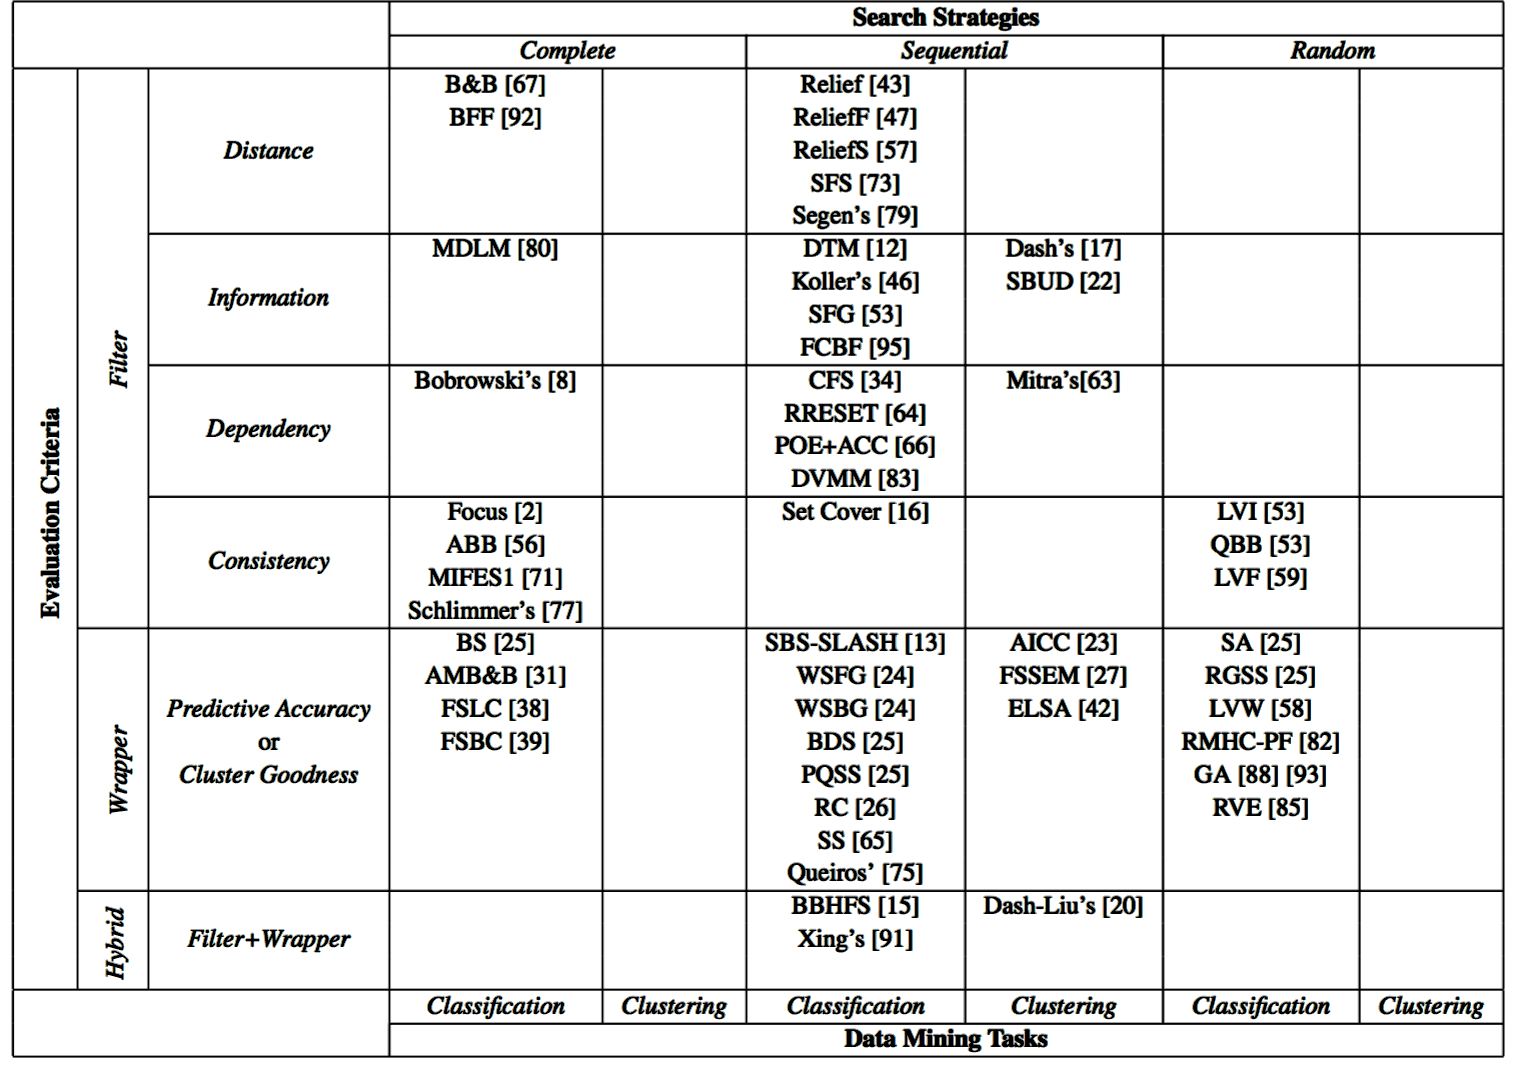
\includegraphics[scale=0.3]{img/img2-categorization-3d}
	\caption{Categorization of feature selection algorithms (Source: \cite{Liu:2005})} \label{fig:img2}
\end{figure}

Feature selection algorithms are categorized in three-dimensional framework in \cite{Liu:2005}. The three dimensions are evaluation criteria, search strategies and data mining tasks on which algorithms are more suitable to perform. We based our algorithms list on the categorization in Figure \ref{fig:img2} and added more up-to-date algorithms to the list.


%Beam search: complete search. sequential search adding (or removing) $p$ features in one step and removing (or adding) $q$ features in the next step $(p>q)$.

\subsection{Filter Methods}\label{ch2:alg:fil}

\begin{itemize}

\item Branch and Bound algorithm (B\&B) 
\newline B\&B \cite{Narendra:1977} is a search algorithm proposed in 1977. It is a depth-first-search tree-based feature elimination strategy, by evaluating the criterion at each level and sort them, continued with pruning. The advantage of this algorithm is: it guarantees that the selected subset yields the globally best value of any criterion that satisfies monotonicity. However, as it performs the full complete search, the number of subsets evaluated can be huge as the number of features grow. The complexity of the algorithm could grow to exponential.

\item Best First strategy for feature selection (BFF)
\newline BFF \cite{Xu:1988} was proposed as an improvement of B\&B algorithm. It is a heuristic search strategy that guarantee the globally best subset without exhaustive enumeration for any criterion that satisfies monotonicity. The advantage is that the number of subsets evaluated by BFF is less than those needed by B\&B algorithm. However, the complexity of the algorithm remains to be exponential as it utilizes  graph and compute the path to select subsets.

\item Relief
\newline Relief algorithm selects relevant features using a statistical method, does not depend on heuristics, is accurate even if features interact, and is noise-tolerant \cite{Kira:1992}. For each randomly selected instance, find nearest hit and miss to determine quality estimation. It can deal with nominal and numerical attributes, but it cannot deal with incomplete data and is limited to two-class problems. The complexity of this algorithm is $O(kN^2)$ (quadratic).

\item ReliefF
\newline ReliefF algorithm \cite{Kononenko:1994} is an variant of improvements of Relief algorithm. ReliefF tries to overcome Relief algorithm's limitation on handling only binary classes. ReliefF handles multiple classes and incomplete and noisy data. For each randomly selected instance, find nearest hit from the same class. For neighbours that are not in the same class, compute the miss. Update quality estimation for each attribute based on those difference. The complexity of the algorithm is improved to $O(kN)$, however, the optimal results are not guaranteed.

\item RReliefF
\newline ReliefF was further extended to RReliefF in order to handle continuous classes in regression. \cite{Robnik-Sikonja:1997} shows that RReliefF is effective in selecting features in learning regression trees for regression problems.

\item Relief with selective sampling (ReliefS)
\newline ReliefS was proposed on 2004 \cite{Liu:2004} as the improvement of Relief algorithm, which creates $kd$-tree upon each bucket of features and adds random sampling. The algorithm in Figure \ref{fig:img5} shows that ReliefS used either sample size $m$ or bucket size $t$ to control the $kd$-tree splitting process. With $N$ number of instances, $t = N/m$. Therefore, if $m$ is predetermined, the splitting process stops when it reaches the level where each bucket contains $N/m$ or fewer instances.  \cite{Liu:2004} also shows that ReliefS in general achieves better performance than ReliefF in terms of learning accuracy and hence selective sampling is an effective approach for active feature selection.

\begin{figure}
	\centering
	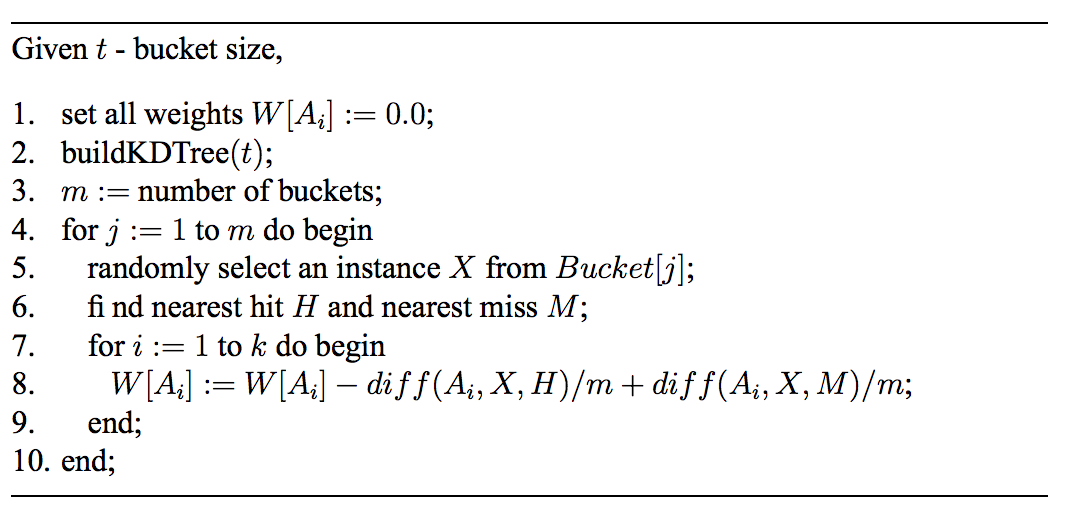
\includegraphics[scale=0.80]{img/img5-reliefs-pseudocode}
	\caption{Relief with selective sampling algorithm} \label{fig:img5}
\end{figure}

\item Sequential Feature Selection (SFS)
\newline Adds one feature which gives the highest value for the objective function, then the remaining features are added individually to the current subset and the new subset is evaluated. The individual feature is permanently included in the subset if it gives the maximum classification accuracy. The process is repeated until the required number of features are added. This is a naive SFS algorithm since the dependency between the features is not accounted for. The complexity of this algorithm is quadratic.

\item Sequential Floating Feature Selection (SFFS)
\newline This algorithm was proposed as an improvement of SFS algorithm. This algorithm works similarly to SFS but in addition, it adds another step which excludes one feature at a time from the subset obtained in the first step and evaluates the new subsets. The complexity of the algorithm remains to be quadratic.

\item Sequential Backward Selection (SBS)
\newline This algorithm works the same way as SFS algorithm, but it starts from a full set and removes a feature on each step. The process is repeated until the required number of features needed is achieved. The complexity of this algorithm is quadratic.

\end{itemize}


\subsection{Wrapper Methods}\label{ch2:alg:wra}

Wrapper methods are broadly classified into sequential selection algorithms and heuristic search algorithms \cite{Chandrashekar:2014}.

\begin{itemize}
\item Particle Swarm Optimization (PSO)
\newline This algorithm yields local optimum results are employed which can produce good results and are computationally feasible.
\item Genetic Algorithm (GA)
\newline This algorithm \cite{Yang:1998} also yields local optimum results are employed which can produce good results and are computationally feasible.
\end{itemize}

%The sequential selection algorithms start with an empty set (full set) and add features (remove features) until the maximum objective function is obtained. To speed up the selection, a criteria is chosen which incrementally increases the objective function until the maximum is reached with the minimum number of features. The heuristic search algorithms evaluate different subsets to optimize the objective function. Different subsets are generated either by searching around in a search- space or by generating solutions to the optimization problem. First we will look at sequential selection algorithms followed by the heuristic search algorithms.

\subsection{Embedded Methods}\label{ch2:alg:emb}

\begin{itemize}
\item Boosting Based Hybrid Feature Selection (BBHFS)
%\newline A major problem of forward selection methods is that it is difficult for them to select sets of features that are good copredictors of the class if none of these predictors is a good predictor of the class by itself.
\end{itemize}

\section{Parallel Algorithms}\label{ch2:par}


\section{Selected Algorithm}\label{ch2:sel}

\appendix
\chapter{Tables}

\begin{table}
\caption{Armadillos}
\label{arm:table}
\begin{center}
\begin{tabular}{||l|l||}\hline
Armadillos & are \\\hline
our	   & friends \\\hline
\end{tabular}
\end{center}
\end{table}

\clearpage
\newpage

\chapter{Figures}

\vspace*{-3in}

\begin{figure}
\vspace{2.4in}
\caption{Armadillo slaying lawyer.}
\label{arm:fig1}
\end{figure}
\clearpage
\newpage

\begin{figure}
\vspace{2.4in}
\caption{Armadillo eradicating national debt.}
\label{arm:fig2}
\end{figure}
\clearpage
\newpage

%% This defines the bibliography file (main.bib) and the bibliography style.
%% If you want to create a bibliography file by hand, change the contents of
%% this file to a `thebibliography' environment.  For more information 
%% see section 4.3 of the LaTeX manual.
\begin{singlespace}
\bibliography{main}
\bibliographystyle{plain}
\end{singlespace}

\end{document}

